 Inicialmente, o objetivo era construir uma aplicação completa para gestão de vendas, focando na geração do pedido e entrega, sendo essa para qualquer ramo de atividade. Porém descobriu-se a possibilidade de um nicho de mercado ainda não explorado e sem concorrentes, em que não é preciso disputar clientes com grandes empresas renomadas e maduras no assunto.
 
 A aplicação desenvolvida foca no gerenciamento das rotas de entregas dos pedidos gerados via e-PDV já operantes, necessitando apenas da disponibilização de uma API no formato de arquivo JSON (\autoref{fig:drHttpAPI}), essa compondo-se de dados essenciais para realização da integração automática abordada na próxima Seção.
 
  \begin{figure}[H]
    \centering
    \caption{Delivery Routes - Requisição HTTP}
    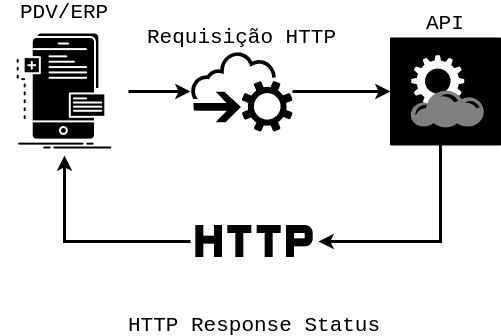
\includegraphics[width=0.6\textwidth]{./dados/figuras/fig16}
    \fonte{\citeonline{iFood}}
    \label{fig:drHttpAPI}
\end{figure}
 
 Primeiramente é preciso entender os possíveis status e o fluxo de um pedido integrado na Delivery Routes, ambos representados na \autoref{tab:drStatusPedido} e na \autoref{fig:drStatusPedido}.
 
 \begin{table}[H]
    \centering
    \caption{Delivery Routes - Status do pedido
    \label{tab:drStatusPedido}}
\begin{tabular}{|l|l|}
\hline
\textbf{Status} & \textbf{Descrição} \\ \hline
PLACED & Indica um pedido foi colocado no sistema. \\ \hline
CONFIRMED & Indica um pedido confirmado. \\ \hline
INTEGRATED & Indica um pedido que foi integrado no sistema. \\ \hline
CANCELLED & Indica um pedido que foi cancelado. \\ \hline
DISPATCHED & Indica um pedido que foi despachado ao cliente. \\ \hline
DELIVERED & Indica um pedido que foi entregue. \\ \hline
CONCLUDED & Indica um pedido que foi concluído. \\ \hline
\end{tabular}
    \fonte{\citeonline{iFood}}
\end{table}
 
 \begin{figure}[H]
    \centering
    \caption{Delivery Routes - Fluxo do status do pedido}
    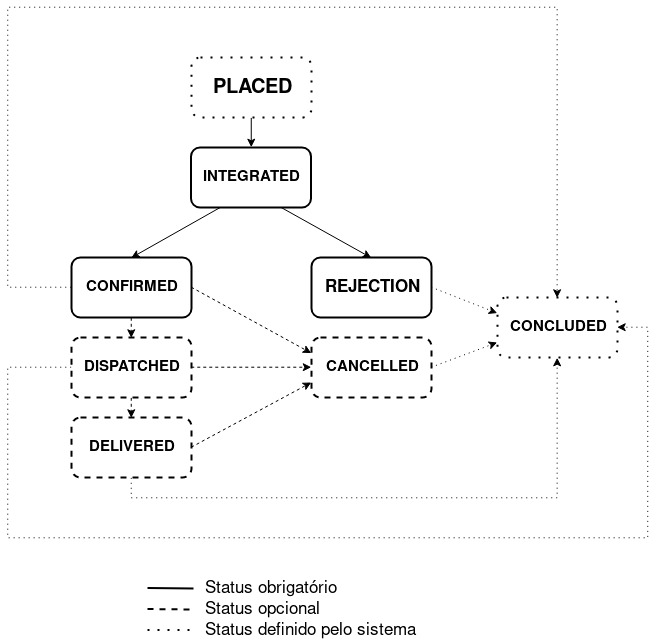
\includegraphics[width=0.6\textwidth]{./dados/figuras/fig15}
    \fonte{\citeonline{iFood}}
    \label{fig:drStatusPedido}
\end{figure}

%%%Se o valor da coluna token_access é diferente ao hash da sessão siginfica que o usuário fez um novo login e gerou um novo hash. Neste caso podemos deslogar o usuário, caso os valores não se coinsidam.

Na \autoref{fig:drLogin} é possível visualizar o acesso ao módulo de gerenciamento, com autenticação apenas para administradores, realizada via e-mail e senha, cujo cadastro é efetuado por meio do link \textit{Register a new membership}. Habilitando a opção \textit{Remember Me}, o controle de única sessão por usuário é ativado, por intermédio de um \textit{hash} gerado no momento do login. É disponibilizado também o link \textit{I forgot my password} para realizar a recuperação da senha, mediante a confirmação de um e-mail existente na base de dados.

\begin{figure}[H]
    \centering
    \caption{Delivery Routes - Login}
    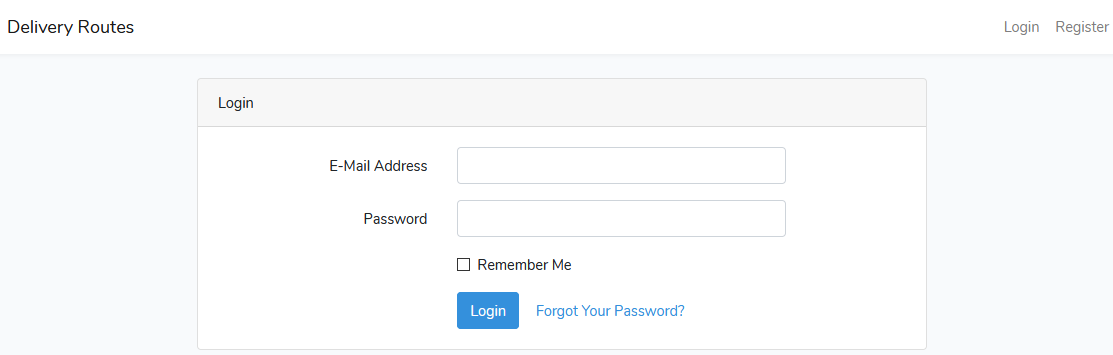
\includegraphics[width=0.4\textwidth]{./dados/figuras/fig7}
    \fonte{Autor}
    \label{fig:drLogin}
\end{figure}

%https://laravel.com/docs/5.7/hashing
O Laravel, juntamente com o Eloquent, disponibiliza a implementação de autenticação de maneira muito simples, por meio do comando \textit{php artisan make:auth}, onde, com poucas instruções e linhas de código, é possível montar a estrutura de cadastro de usuário, recuperação de senha e memória de sessão de maneira extremamente segura, devido ao algoritmo \textit{Bcrypt}
\footnote{Método de criptografia do tipo \textit{hash} adaptativo para senhas que apresenta uma segurança maior em relação à maioria dos outros métodos criptográficos por meio da implementação da variável “custo”, que é proporcional à quantidade de processamento necessária para criptografar a senha \cite{bcrypt}.}
, utilizado para realizar a criptografia da senha.

Ao realizar login, o administrador é apresentado à \textit{dashboard} do sistema, uma interface gráfica que fornece visualização fácil e rápida dos principais indicadores de desempenho, atualizados em tempo real, obtendo assim valores e médias relevantes sobre o processo de negócios. 

Destaca-se na \autoref{fig:drDashboard}, além de indicadores de: Pedidos Em Aberto, Pedidos Em Rota, Motoboys Disponíveis e Pedidos Concluídos, uma barra de menus contendo: Cadastros (Motoboys e Pagamentos) e Movimentos (Entregas e Pedidos Em Aberto).

\begin{figure}[H]
    \centering
    \caption{Delivery Routes - Dashboard}
    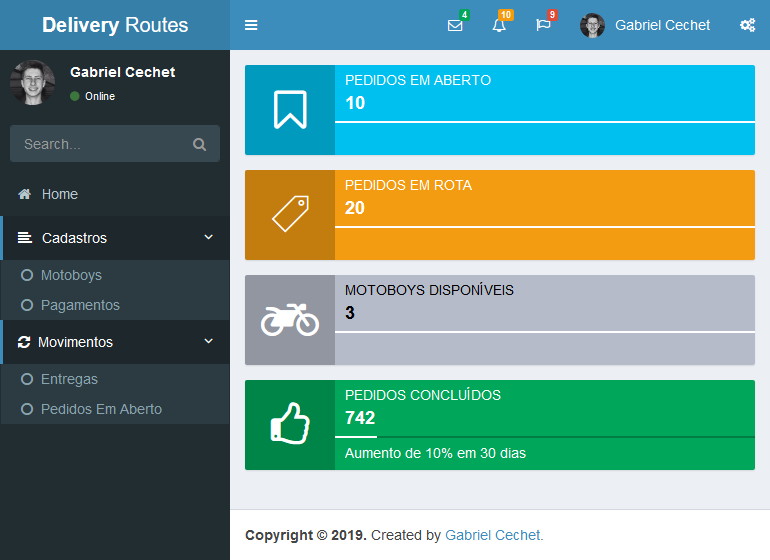
\includegraphics[width=1.0\textwidth]{./dados/figuras/fig13}
    \fonte{Autor}
    \label{fig:drDashboard}
\end{figure}

\newpage
Para desenvolver a \textit{dashboard}
%%% Rev-Madalozzo: listar todos os pacotes de terceiros AdminLTE e PDF
